% Options for packages loaded elsewhere
\PassOptionsToPackage{unicode}{hyperref}
\PassOptionsToPackage{hyphens}{url}
%
\documentclass[
]{article}
\usepackage{lmodern}
\usepackage{amssymb,amsmath}
\usepackage{ifxetex,ifluatex}
\ifnum 0\ifxetex 1\fi\ifluatex 1\fi=0 % if pdftex
  \usepackage[T1]{fontenc}
  \usepackage[utf8]{inputenc}
  \usepackage{textcomp} % provide euro and other symbols
\else % if luatex or xetex
  \usepackage{unicode-math}
  \defaultfontfeatures{Scale=MatchLowercase}
  \defaultfontfeatures[\rmfamily]{Ligatures=TeX,Scale=1}
\fi
% Use upquote if available, for straight quotes in verbatim environments
\IfFileExists{upquote.sty}{\usepackage{upquote}}{}
\IfFileExists{microtype.sty}{% use microtype if available
  \usepackage[]{microtype}
  \UseMicrotypeSet[protrusion]{basicmath} % disable protrusion for tt fonts
}{}
\makeatletter
\@ifundefined{KOMAClassName}{% if non-KOMA class
  \IfFileExists{parskip.sty}{%
    \usepackage{parskip}
  }{% else
    \setlength{\parindent}{0pt}
    \setlength{\parskip}{6pt plus 2pt minus 1pt}}
}{% if KOMA class
  \KOMAoptions{parskip=half}}
\makeatother
\usepackage{xcolor}
\IfFileExists{xurl.sty}{\usepackage{xurl}}{} % add URL line breaks if available
\IfFileExists{bookmark.sty}{\usepackage{bookmark}}{\usepackage{hyperref}}
\hypersetup{
  pdftitle={Taller Final: muestreo estadístico},
  pdfauthor={Julián Camilo Riaño Moreno},
  hidelinks,
  pdfcreator={LaTeX via pandoc}}
\urlstyle{same} % disable monospaced font for URLs
\usepackage[margin=1in]{geometry}
\usepackage{graphicx,grffile}
\makeatletter
\def\maxwidth{\ifdim\Gin@nat@width>\linewidth\linewidth\else\Gin@nat@width\fi}
\def\maxheight{\ifdim\Gin@nat@height>\textheight\textheight\else\Gin@nat@height\fi}
\makeatother
% Scale images if necessary, so that they will not overflow the page
% margins by default, and it is still possible to overwrite the defaults
% using explicit options in \includegraphics[width, height, ...]{}
\setkeys{Gin}{width=\maxwidth,height=\maxheight,keepaspectratio}
% Set default figure placement to htbp
\makeatletter
\def\fps@figure{htbp}
\makeatother
\setlength{\emergencystretch}{3em} % prevent overfull lines
\providecommand{\tightlist}{%
  \setlength{\itemsep}{0pt}\setlength{\parskip}{0pt}}
\setcounter{secnumdepth}{-\maxdimen} % remove section numbering
\usepackage{float}
\floatplacement{figure}{H}
\usepackage{booktabs}
\usepackage{booktabs}
\usepackage{longtable}
\usepackage{array}
\usepackage{multirow}
\usepackage{wrapfig}
\usepackage{float}
\usepackage{colortbl}
\usepackage{pdflscape}
\usepackage{tabu}
\usepackage{threeparttable}
\usepackage{threeparttablex}
\usepackage[normalem]{ulem}
\usepackage{makecell}
\usepackage{xcolor}

\title{Taller Final: muestreo estadístico}
\usepackage{etoolbox}
\makeatletter
\providecommand{\subtitle}[1]{% add subtitle to \maketitle
  \apptocmd{\@title}{\par {\large #1 \par}}{}{}
}
\makeatother
\subtitle{Muestreo aleatorio estratificado}
\author{Julián Camilo Riaño Moreno}
\date{domingo, junio 28, 2020}

\begin{document}
\maketitle

{
\setcounter{tocdepth}{2}
\tableofcontents
}
\hypertarget{actividad}{%
\section{Actividad}\label{actividad}}

\begin{quote}
El objetivo de esta actividad es hacer un diseño muestral estratificado,
según lo visto en clase.
\end{quote}

\begin{itemize}
\tightlist
\item
  Se debe seleccionar una base, puede ser una base propia o la base de
  wine+quality.
\item
  Seleccione una única variable para hacer los niveles de
  estratificación.
\item
  Realice una prueba piloto.
\item
  Defina cuál debe ser el tamaño de la muestra total y de casa uno de
  los estratos.
\item
  De algunas conclusiones de los resultados.
\item
  Se debe subir la actividad antes del 29 de junio a las 23:59 horas.
\item
  Debe subirse en un archivo pdf.
\end{itemize}

\hypertarget{especificaciones-base-de-datos-y-adecuaciones}{%
\subsection{Especificaciones base de datos y
adecuaciones}\label{especificaciones-base-de-datos-y-adecuaciones}}

\begin{quote}
Este conjunto de datos también está disponible en el repositorio de
aprendizaje automático de {[}UCI (Universidad de California en
Irvine){]},
(\url{https://archive.ics.uci.edu/ml/datasets/wine+quality}). Estos
conjuntos de datos están relacionados con variantes rojas del vino
portugués ``Vinho Verde''. Para más detalles, consulte la referencia
{[}Cortez et al., 2009{]}.
\end{quote}

\begin{quote}
Variables de entrada (basadas en pruebas fisicoquímicas):
\end{quote}

\begin{enumerate}
\def\labelenumi{\arabic{enumi}.}
\tightlist
\item
  fixed acidity
\item
  volatile acidity
\item
  citric acid
\item
  residual sugar
\item
  chlorides
\item
  free sulfur dioxide
\item
  total sulfur dioxide
\item
  density
\item
  pH
\item
  sulphates
\item
  alcohol
\item
  quality (score between 0 and 10)
\end{enumerate}

Con el fin de realizar el análisis de muestreo estratificado por dos
métodos (muestreo aleatorio estratificado y muestro estratificado de
Neyman), se decide definir una cualificacion del vino elegido (para este
caso eligió la base de datos de vino blaco). La cualificación designada
fue la escala de ``dulzor del vino'' para definir esto acudió a la
{[}escala de Rieseling{]}
(\url{https://drinkriesling.com/tasteprofile/thescale}).

Esta clasificación se define a través de la relación entre azucares
residuales y ácidos del vino. Por esta razón, se decidió realizar una
nueva columna en la base de datos que corresponde al \emph{indice de
Rieseling} a través de la siguiente relación:

\[
IRF\ Rieseling = \frac{residual\_sugar} {fixed\_ acidity+volatile\_ acidity+citric\_ acid}
\] Posteriormente ya obtenida esta nueva columna en la base de datos se
decidió realizar una asignación de categorías para los vino con relación
a este indice de la siguiente manera:

\begin{itemize}
\tightlist
\item
  IRF Rieseling \(< 1.0\) = dry (seco)
\item
  IRF Rieseling \(1.0 - 2.0\) = semi\_dry (semi-seco)
\item
  IRF Rieseling \(2.1 - 4.0\) = semi\_sweet (semi-dulce)
\item
  IRF Rieseling \(> 4.0\) = sweet (dulce)
\end{itemize}

Al aplicar esta categorización se encontró que solo una observación
correspondía a \texttt{sweet}, de manera que se decidió eliminar porque
no aportaba al análisis. De esta forma, los vinos se categorizaron
únicamente en \texttt{dry} (seco), \texttt{semi-dry} (semi-seco),
\texttt{semi-sweet} (semi-dulce), estos fueron lo estratos que se
definieron para este estudio.

\hypertarget{muestreo-aleatorio-estratificado}{%
\section{Muestreo aleatorio
estratificado}\label{muestreo-aleatorio-estratificado}}

\hypertarget{datos-iniciales-y-estimadores-para-cada-variable.}{%
\subsection{Datos iniciales y estimadores para cada
variable.}\label{datos-iniciales-y-estimadores-para-cada-variable.}}

El primer análisis realizado fue un muestreo aleatorio estratificado
simple; en el cual se utilizó unicamente la función \texttt{sample} del
paquete básico de \emph{R}. Además se realizó el análisis para estimar
los tamaños de muestra esperado para cada una de las 12 variables de la
base de datos. Para todos los análisis de este metodo se definió un
error estandar de 0.05 y un nivel de confianza de 0.95.

Inicialmente se realizó una determinación de muestra para el estudio
piloto y se definió un posible tamaño de muestra para cada uno de los
estratos para la muestra piloto. Para esto se tuvo en cuenta que la
categorización se realizó a partir de los 3 estratos antes comentados
(ver tabla 1.)

\begin{table}[!h]

\caption{\label{tab:tabla_piloto_total}Tamaños de población y muestras (piloto y estratos)}
\centering
\fontsize{8}{10}\selectfont
\begin{tabular}[t]{c|c|c}
\hline
N & n piloto & n estratos\\
\hline
\rowcolor{gray!6}  4897 & 245 & 81.667\\
\hline
\multicolumn{3}{l}{\textit{Note: }}\\
\multicolumn{3}{l}{Para el n del piloto se utilizo un error = 0.05}\\
\end{tabular}
\end{table}

La tabla 2. muestra los estimadores para la muestra piloto para cada una
de las variables organizadas por estrato.

Posteriormente se decidió obtener las proporciones para cada de los
muestreos para cada una de los estratos, como se muestra la tabla 3. A
partir de estos datos, se encuentra que la mayor proporcion de tamaño
muestral corresponde al estrato \texttt{dry} y el de menor proporción es
el \texttt{semi-sweet}. Se decidió ajustar los estimadores de cada una
de las variables por estrato para cada una de las variables.

\hypertarget{proporciones-y-estimadores-por-estrato}{%
\subsection{Proporciones y estimadores por
estrato}\label{proporciones-y-estimadores-por-estrato}}

\begin{table}[!h]

\caption{\label{tab:gráfica prueba}Estimadores de la muestra piloto}
\centering
\fontsize{6}{8}\selectfont
\begin{tabular}[t]{lrrrrrrrrr}
\toprule
\multicolumn{1}{c}{} & \multicolumn{3}{c}{Media} & \multicolumn{3}{c}{Desviacion estandar} & \multicolumn{3}{c}{Coeficiente de variación} \\
\cmidrule(l{3pt}r{3pt}){2-4} \cmidrule(l{3pt}r{3pt}){5-7} \cmidrule(l{3pt}r{3pt}){8-10}
  & Seco & Semi\_seco & Semi\_dulce & Seco & Semi\_seco & Semi\_dulce & Seco & Semi\_seco & Semi\_dulce\\
\midrule
\rowcolor{gray!6}  fixed.acidity & 6.825 & 7.042 & 6.646 & 0.924 & 0.858 & 0.662 & 0.135 & 0.122 & 0.100\\
volatile.acidity & 0.257 & 0.282 & 0.270 & 0.092 & 0.092 & 0.064 & 0.360 & 0.325 & 0.236\\
\rowcolor{gray!6}  citric.acid & 0.336 & 0.346 & 0.325 & 0.103 & 0.119 & 0.129 & 0.307 & 0.344 & 0.398\\
residual.sugar & 2.986 & 11.148 & 17.562 & 2.010 & 2.737 & 2.138 & 0.673 & 0.245 & 0.122\\
\rowcolor{gray!6}  chlorides & 0.042 & 0.046 & 0.051 & 0.016 & 0.011 & 0.013 & 0.374 & 0.234 & 0.247\\
\addlinespace
free.sulfur.dioxide & 28.778 & 42.506 & 40.765 & 14.413 & 17.981 & 14.529 & 0.501 & 0.423 & 0.356\\
\rowcolor{gray!6}  total.sulfur.dioxide & 118.735 & 162.383 & 158.185 & 38.468 & 49.181 & 38.063 & 0.324 & 0.303 & 0.241\\
density & 0.992 & 0.996 & 0.999 & 0.002 & 0.002 & 0.002 & 0.002 & 0.002 & 0.002\\
\rowcolor{gray!6}  pH & 3.176 & 3.118 & 3.150 & 0.153 & 0.133 & 0.131 & 0.048 & 0.043 & 0.042\\
sulphates & 0.470 & 0.483 & 0.469 & 0.113 & 0.112 & 0.062 & 0.239 & 0.232 & 0.133\\
\addlinespace
\rowcolor{gray!6}  alcohol & 11.086 & 9.792 & 9.321 & 1.125 & 0.877 & 0.747 & 0.101 & 0.090 & 0.080\\
quality & 6.049 & 5.790 & 5.506 & 0.907 & 0.786 & 0.573 & 0.150 & 0.136 & 0.104\\
\bottomrule
\end{tabular}
\end{table}

La tabla 4. muestra el ajuste de estimadores de los estimadores la
proporción de cada uno de los estratos por variable, y se obtiene el
valor de error estandar para cada una de las variables a partir del
ajuste proporcional.

\begin{table}[!h]

\caption{\label{tab:gráfica prueba_def med ponderada2}Proporciones para cada estrato}
\centering
\fontsize{8}{10}\selectfont
\begin{tabular}[t]{l|c|c|c}
\hline
  & n & N & proporcion\_estrato\\
\hline
\rowcolor{gray!6}  Seco & 3053 & 4897 & 0.623\\
\hline
Semi\_seco & 1591 & 4897 & 0.325\\
\hline
\rowcolor{gray!6}  Semi\_dulce & 253 & 4897 & 0.052\\
\hline
\multicolumn{4}{l}{\textit{Note: }}\\
\multicolumn{4}{l}{Proporción por estrato obtiene de n/N}\\
\end{tabular}
\end{table}

A partir de este valor de error se decidió realizar un analisis de
estimaciones de tamaños de población para cada una de la variables de
manera proporcional. Como se observa en la tabla 5. se obtuvo un tamaño
de muestra para cada una población finita y una población infinita para
cada una de las variables en la segunda parte de la tabla se observa el
valor de n (muestra) para cada una de las variables ajustada al peso de
cada uno de los estratos y el número de n (muestra) final para todas las
variables.

\begin{table}[!h]

\caption{\label{tab:gráfica prueba med_ponderada variable}Medias estratificadas por variable}
\centering
\fontsize{8}{10}\selectfont
\begin{tabular}[t]{lrrrrrrrr}
\toprule
\multicolumn{1}{c}{} & \multicolumn{3}{c}{Media} & \multicolumn{3}{c}{Media ponderada por estrato} & \multicolumn{1}{c}{} & \multicolumn{1}{c}{} \\
\cmidrule(l{3pt}r{3pt}){2-4} \cmidrule(l{3pt}r{3pt}){5-7}
  & Seco & Semi\_seco & Semi\_dulce & Seco & Semi\_seco & Semi\_dulce & Media estratificada & Error\\
\midrule
\rowcolor{gray!6}  fixed.acidity & 6.825 & 7.042 & 6.646 & 4.255 & 2.288 & 0.343 & 6.886 & 0.344\\
volatile.acidity & 0.257 & 0.282 & 0.270 & 0.160 & 0.092 & 0.014 & 0.266 & 0.013\\
\rowcolor{gray!6}  citric.acid & 0.336 & 0.346 & 0.325 & 0.210 & 0.113 & 0.017 & 0.339 & 0.017\\
residual.sugar & 2.986 & 11.148 & 17.562 & 1.862 & 3.622 & 0.907 & 6.391 & 0.320\\
\rowcolor{gray!6}  chlorides & 0.042 & 0.046 & 0.051 & 0.026 & 0.015 & 0.003 & 0.043 & 0.002\\
\addlinespace
free.sulfur.dioxide & 28.778 & 42.506 & 40.765 & 17.941 & 13.810 & 2.106 & 33.857 & 1.693\\
\rowcolor{gray!6}  total.sulfur.dioxide & 118.735 & 162.383 & 158.185 & 74.024 & 52.757 & 8.173 & 134.954 & 6.748\\
density & 0.992 & 0.996 & 0.999 & 0.618 & 0.324 & 0.052 & 0.994 & 0.050\\
\rowcolor{gray!6}  pH & 3.176 & 3.118 & 3.150 & 1.980 & 1.013 & 0.163 & 3.156 & 0.158\\
sulphates & 0.470 & 0.483 & 0.469 & 0.293 & 0.157 & 0.024 & 0.474 & 0.024\\
\addlinespace
\rowcolor{gray!6}  alcohol & 11.086 & 9.792 & 9.321 & 6.911 & 3.181 & 0.482 & 10.574 & 0.529\\
quality & 6.049 & 5.790 & 5.506 & 3.771 & 1.881 & 0.284 & 5.937 & 0.297\\
\bottomrule
\end{tabular}
\end{table}

Estos valores de n finales obtenidos para cada una de las variables,
están ajustados para cada uno de los errores por variable. No se realizó
análisis de margenes de errores. Sin embargo, de esta tabla se puede
observar como aquellas variables que presentan valores más cercanos a la
media, o más consistentes (con menor varianza) son los que menor número
de muestra requieren por ejemplo \texttt{density} arroja un valor de 0
al redondearlo, lo cual es incomprensible. Sin embargo, si se observa el
número en decimal se obtiene que con aproximadamente 1 solo indviduo
muestreado se obtendra información sobre esta variable; esto se debe a
la poca varianza y bajo error que presenta esta variable. No obstante,
esto no permite realizar un análisis más profundo de las muestras por
estrato. De manera que, para el siguiente punto se decidió utilizar una
única variable que presentara mayor varianza \texttt{citric.acid}.

\begin{table}[!h]

\caption{\label{tab:tabla_errores_varall}Tamaños de muestra definidos por error de cada variable para población finita e infinita y proporciones finales por estrato}
\centering
\fontsize{8}{10}\selectfont
\begin{tabular}[t]{lrrrrrrr}
\toprule
\multicolumn{1}{c}{ } & \multicolumn{1}{c}{} & \multicolumn{2}{c}{Prueba para tipo de población} & \multicolumn{3}{c}{Valor de n proporcionada por estrato} & \multicolumn{1}{c}{} \\
\cmidrule(l{3pt}r{3pt}){3-4} \cmidrule(l{3pt}r{3pt}){5-7}
  & Error & P\_infinite & P\_finite & Seco & Semi\_seco & Semi\_dulce & n\_final\\
\midrule
\rowcolor{gray!6}  fixed.acidity & 0.3443 & 25.7517 & 25.6170 & 16 & 8 & 1 & 25\\
volatile.acidity & 0.0133 & 180.1221 & 173.7318 & 108 & 56 & 9 & 173\\
\rowcolor{gray!6}  citric.acid & 0.0169 & 162.2572 & 157.0534 & 98 & 51 & 8 & 157\\
residual.sugar & 0.3195 & 195.1691 & 187.6888 & 117 & 61 & 10 & 188\\
\rowcolor{gray!6}  chlorides & 0.0022 & 159.7650 & 154.7173 & 96 & 50 & 8 & 154\\
\addlinespace
free.sulfur.dioxide & 1.6929 & 329.0141 & 308.3004 & 192 & 100 & 16 & 308\\
\rowcolor{gray!6}  total.sulfur.dioxide & 6.7477 & 150.4530 & 145.9683 & 91 & 47 & 8 & 146\\
density & 0.0497 & 0.0061 & 0.0061 & 0 & 0 & 0 & 0\\
\rowcolor{gray!6}  pH & 0.1578 & 3.2834 & 3.2812 & 2 & 1 & 0 & 3\\
sulphates & 0.0237 & 83.2737 & 81.8813 & 51 & 27 & 4 & 82\\
\addlinespace
\rowcolor{gray!6}  alcohol & 0.5287 & 14.6673 & 14.6235 & 9 & 5 & 1 & 15\\
quality & 0.2969 & 31.8443 & 31.6385 & 20 & 10 & 2 & 32\\
\bottomrule
\multicolumn{8}{l}{\textit{Note: }}\\
\multicolumn{8}{l}{P\_infinite = muestra (n) total para población infinita}\\
\multicolumn{8}{l}{P\_finite = muestra (n) total para población finita}\\
\end{tabular}
\end{table}

\hypertarget{muestreo-estratificado-por-muxe9todo-de-neyman}{%
\section{Muestreo estratificado por método de
Neyman}\label{muestreo-estratificado-por-muxe9todo-de-neyman}}

A través del análisis realizado en el punto anterior se eligió la
variable \texttt{citric.acid}para conducir el muestreo por método de
Neyman con una única variable.

Para iniciar el estudio de muestreo, realizó un análisis descriptivo
iniciarl de la variable para cada uno de los estratos definidos
(\texttt{dry}, \texttt{semi-dry}, \texttt{semi-sweet}). En la figura 1,
se puede evidenciar las proporciones de cada uno de los estratos en la
base de datos original de vino blanco \footnote{se eliminó una
  observación como se comentó anteriormente porque era un dato extremo
  para la escala de Reiseling; la cual sirvió para la estratificación
  realizada.}, esto es \(N = 4897\).

\hypertarget{evaluaciuxf3n-descriptiva-de-la-variable-citric.acid-y-normalizaciuxf3n.}{%
\subsection{\texorpdfstring{Evaluación descriptiva de la variable
\texttt{citric.acid} y
normalización.}{Evaluación descriptiva de la variable citric.acid y normalización.}}\label{evaluaciuxf3n-descriptiva-de-la-variable-citric.acid-y-normalizaciuxf3n.}}

\begin{figure}
\centering
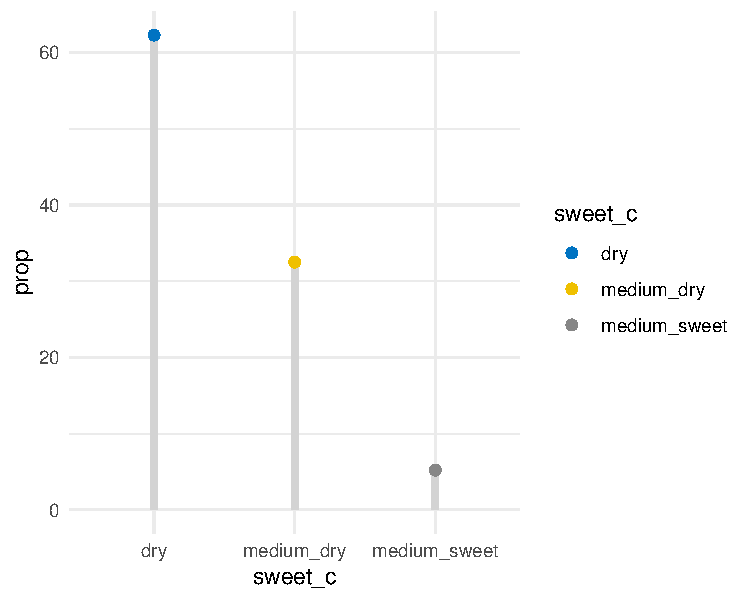
\includegraphics{muestreo_estratificado_final_files/figure-latex/proportion untidy-1.pdf}
\caption{Gráfica de proporciones de los estratos en la base de datos
original}
\end{figure}

Para evaluar la variable \texttt{citric.acid} en los estratos se
realizaron dos graficas (figura 2 y 3), una densidad y otra un BoxPlot,
respectivamente.

\begin{figure}
\centering
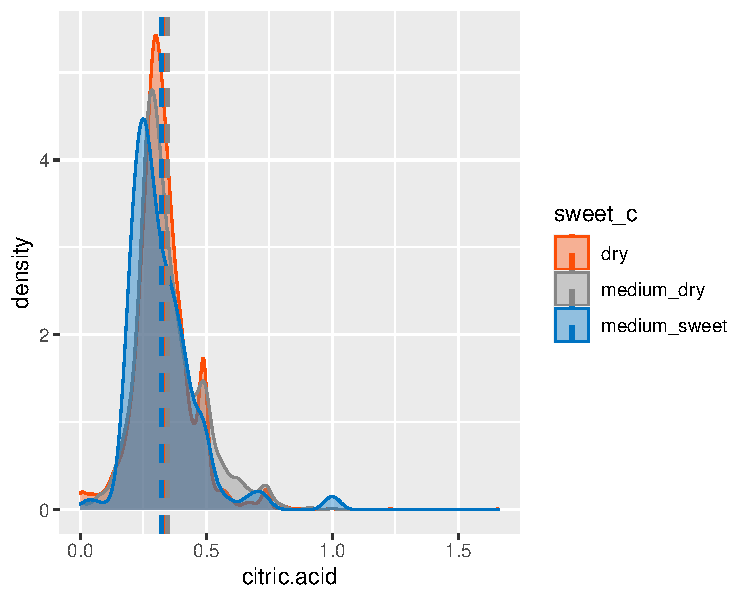
\includegraphics{muestreo_estratificado_final_files/figure-latex/desity_plot untidy-1.pdf}
\caption{Gráfica de densidad de la variable \texttt{citric.acid} por
estrato (las lineas representan los valores de media de la variable
estudiada}
\end{figure}

\begin{figure}
\centering
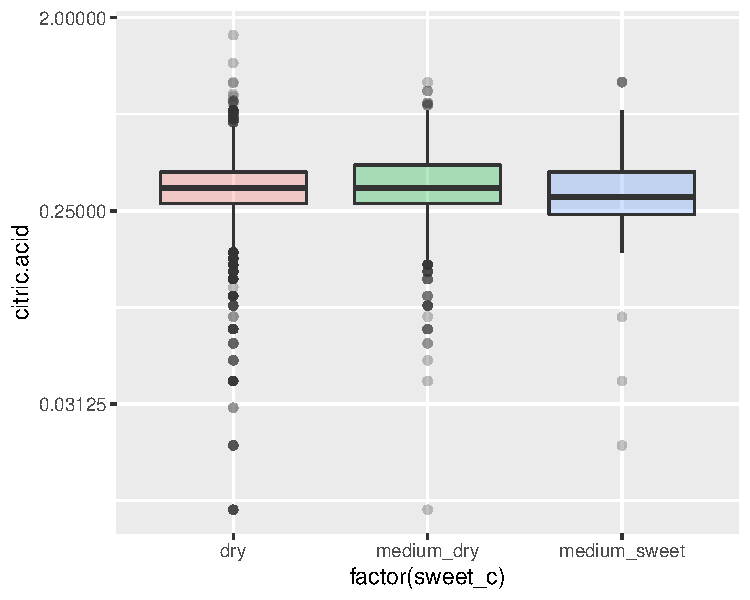
\includegraphics{muestreo_estratificado_final_files/figure-latex/Boxplot untidy-1.pdf}
\caption{Gráfica de Boxplot de la variable \texttt{citric.acid} por
estrato, de la base de datos original}
\end{figure}

Como se puede observaren estas figuras, en primer lugar se observa que
las observaciones para los grupos, en la gráfica de densidad (figura 2)
exhiben una asimetría hacia la izquierda. Lo cual puede ser dado a
múltiples \emph{outliers}. Para verificar esto, se realizó un BoxPlot
(figura 3) en el cual se verifica el gran número de observaciones
\emph{outliners} (debido a los valores tan pequeños de las observaciones
de la variable \texttt{citric.acid} se decidió hacer una transformación
logaritmica (\(log_2\)))

Por lo anterior se decide realizar una limpieza de \emph{outliers}, con
lo cual se eliminan \textbf{269} observaciones. Con lo cual se deja una
nueva base de datos limpia de \(N = 4628\). Para verificar la normalidad
se realiza un nuevo análisis descriptivo.

\begin{figure}
\centering
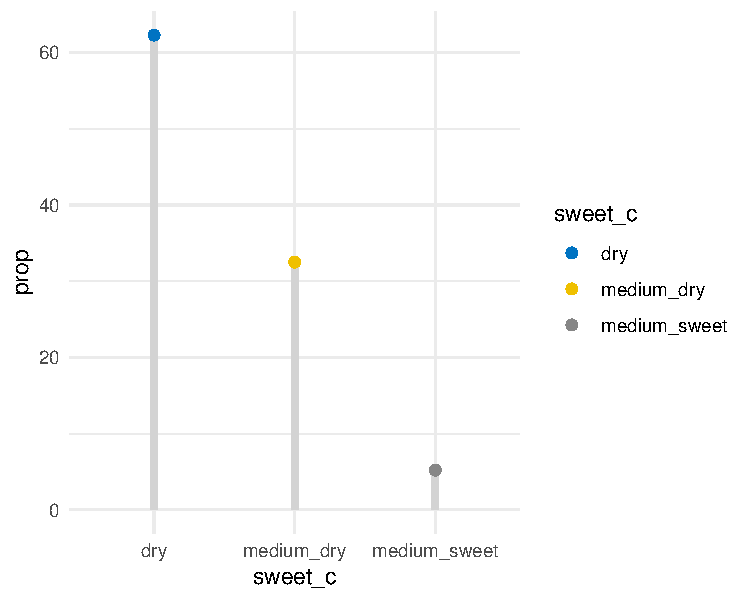
\includegraphics{muestreo_estratificado_final_files/figure-latex/proportion tidy-1.pdf}
\caption{Gráfica de proporciones de los estratos en la base de datos sin
\emph{outliers}}
\end{figure}

Se evaluan proporciones en la figura 4; observando que la eliminación de
variables no impacto grandemente los estratos, ya que la
proporcionalidad es similar a la base original.

\begin{figure}
\centering
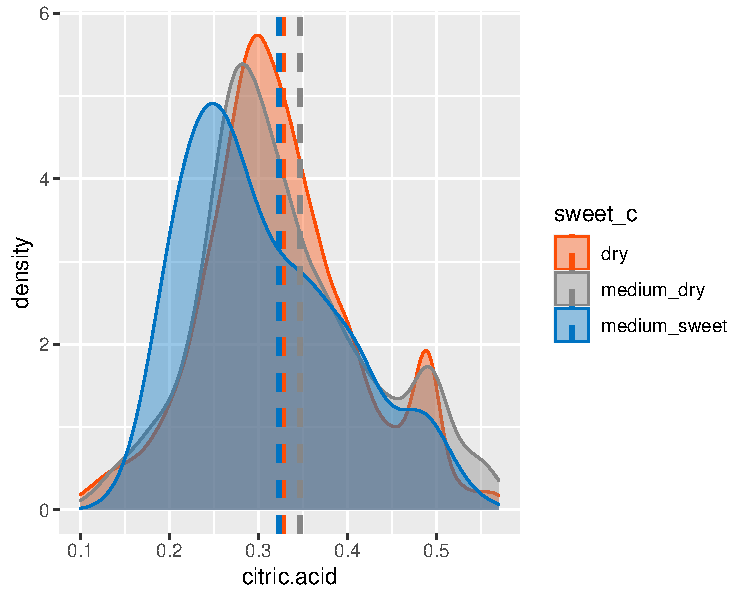
\includegraphics{muestreo_estratificado_final_files/figure-latex/desity_plot tidy-1.pdf}
\caption{Gráfica de densidad de la variable \texttt{citric.acid} por
estrato (las lineas representan los valores de media de la variable
estudiada de la base de datos sin \emph{outliers}}
\end{figure}

\begin{figure}
\centering
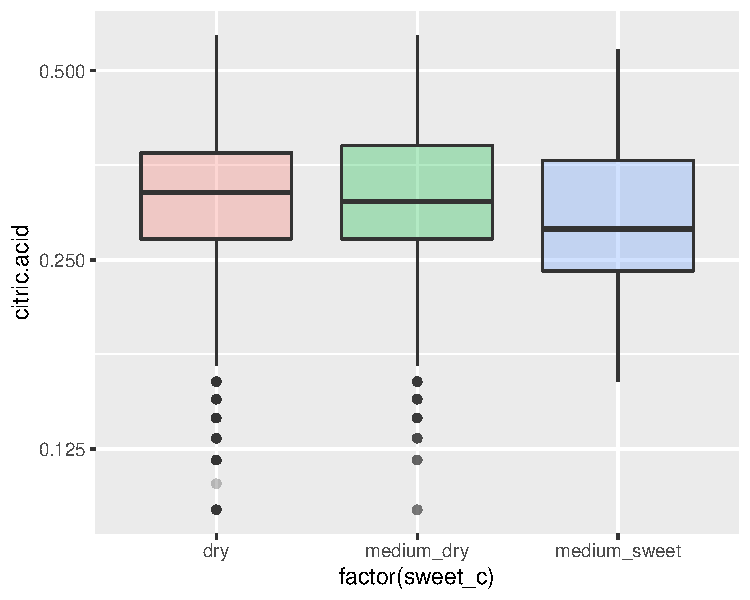
\includegraphics{muestreo_estratificado_final_files/figure-latex/Boxplot tidy-1.pdf}
\caption{Gráfica de Boxplot de la variable \texttt{citric.acid} por
estrato, de la base de datos sin \emph{outliers}}
\end{figure}

Se realiza además una nueva gráfica de densidad (figura 5) y un BoxPlot
(figura 6). Los cuales muestran normalidad en la distribución de las
observaciones y una minimización de \emph{outliers}. Esta nueva base de
datos será la que se utilizará para continuar el análisis de muestreo
por el método de Neyman.

Para los subsiguientes análisis se utilizó un error de 0.05 y nivel de
confianza de 0.95. Incialmente se obtuvo el tamaño de la muestra piloto
a partir del error definido. Estos datos están resumidos en la tabla 6.

\hypertarget{muestra-piloto-y-estimadores}{%
\subsection{muestra piloto y
estimadores}\label{muestra-piloto-y-estimadores}}

\begin{table}[!h]

\caption{\label{tab:tabla 2 inicial}Tamaños de población y muestras piloto}
\centering
\fontsize{8}{10}\selectfont
\begin{tabular}[t]{c|c}
\hline
N & n\_piloto\\
\hline
\rowcolor{gray!6}  4628 & 231\\
\hline
\multicolumn{2}{l}{\textit{Note: }}\\
\multicolumn{2}{l}{Para el n del piloto se utilizo un error = 0.05}\\
\end{tabular}
\end{table}

La tabla 7 corresponde a los valores de n para cada uno de los estratos
desde el N poblacional y el n de la prueba piloto. allí se obtiene a su
vez la desviación estandar de las observaciones para la variable
\texttt{citric.acid} para cada uno de los estratos. Como se puede ver,
el estrato con mayor número de observaciones es \texttt{dry} y el de
menor cantidad de observaciones es \texttt{medium\_sweet}.

\begin{table}[!h]

\caption{\label{tab:n para N y piloto}Tamaños de muestra por estrato para N y el piloto}
\centering
\fontsize{8}{10}\selectfont
\begin{tabular}[t]{c|c|c|c}
\hline
Estrato & Desviacion.Std & n & n total\\
\hline
\rowcolor{gray!6}  dry & 0.086 & 2916 & 140.843\\
\hline
medium\_dry & 0.095 & 1473 & 78.320\\
\hline
\rowcolor{gray!6}  medium\_sweet & 0.088 & 239 & 11.836\\
\hline
\multicolumn{4}{l}{\textit{Note: }}\\
\multicolumn{4}{l}{n total corresponde a la cantidad de observaciones por estrato de n de la prueba piloto}\\
\end{tabular}
\end{table}

Despues de obtenidos los valores de muestra para cada estrato en la
muestra piloto se procedió a aplicar la función \texttt{strata} del
paquete \texttt{sampling}; para obtener las muestras de la base de datos
utilizada para este ejericicio. A partir de este nuevo remuestreo se
obtiene media y varianza de las observaciones resultantes para cada
estrato (ver tabla 8).

\begin{table}[!h]

\caption{\label{tab:media y var strata}Valores de media y varianza para el muestreo por función `strata`}
\centering
\fontsize{8}{10}\selectfont
\begin{tabular}[t]{c|c|c|c}
\hline
Estrato & Media & Varianza & n\_strata\\
\hline
\rowcolor{gray!6}  dry & 0.327 & 0.008 & 140\\
\hline
medium\_dry & 0.322 & 0.009 & 78\\
\hline
\rowcolor{gray!6}  medium\_sweet & 0.326 & 0.008 & 11\\
\hline
\multicolumn{4}{l}{\textit{Note: }}\\
\multicolumn{4}{l}{n strata corresponde al tamaño de n para cada uno}\\
\multicolumn{4}{l}{de los estratos obtenido a traves de la funcion}\\
\multicolumn{4}{l}{[strata] del paquete [sampling]}\\
\end{tabular}
\end{table}

Seguidamente se obtiene los estimadores la variable \texttt{citric.acid}
en la nueva muestra realizada. Además se obtienen unos estimados de
muestra para población finita e infinita a apartir del remuestreo para
toda la base de datos nueva de manera que haya representación de todas
los estratos (tabla 9). Se obtuvo un valor de error (0.016) posible para
la variable y a partir de este se definieron posibles margenes de error
aceptable y se obtuvo sus valores de muestra tanto para población finita
como infinita (esto se puede ver en la tabla 12 al final del documento).

\begin{table}[!h]

\caption{\label{tab:estimadores piloto}Estimadores para la muestra piloto a partit de la variable `citric.acid`}
\centering
\fontsize{8}{10}\selectfont
\begin{tabular}[t]{c|c|c|c|c|c}
\hline
Media\_estimada & N.confianza & Z\_value & Error\_estimado & n\_finita & n\_infinita\\
\hline
\rowcolor{gray!6}  0.325 & 0.95 & -1.96 & 0.016 & 122.974 & 119.791\\
\hline
\multicolumn{6}{l}{\textit{Note: }}\\
\multicolumn{6}{l}{El valor de Z se obtuvo 
                         asumiendo normalidad (media = 0, desviación estandar = 1)}\\
\end{tabular}
\end{table}

\hypertarget{tamauxf1o-de-muestra-para-poblaciuxf3n-infinita-y-finita}{%
\subsection{Tamaño de muestra para población infinita y
finita}\label{tamauxf1o-de-muestra-para-poblaciuxf3n-infinita-y-finita}}

Para observar mejor al relación entre los margenes de error y los
valores de muestra finita e infinita, se decidió realizar gráficas para
comparando los tipos de muestreo. Esto se puede ver en la figura 8. Allí
se puede ver el tamaño de muestra vs el margen de error; sin embargo,
dado que el valor de errores es tan grande y las diferencias entre las
muetras son más diversas en cuato se acerca a 0 el error. Se decidió
realizar una transformación logaritmica de los datos a través de un
logaritmo en base 2 (log2).

La figura 9, muestra la relación entre los errores y las muestras para
población finita e infinita para transformadas logaritmicamente. Como se
puede observar la muestra infinita tiene un comportamiento uniforme, sin
embargo la curva de la muestra para población finita tiene un
aplanamiento cuando está próxima al tamaño de población total (N).

\begin{figure}
\centering
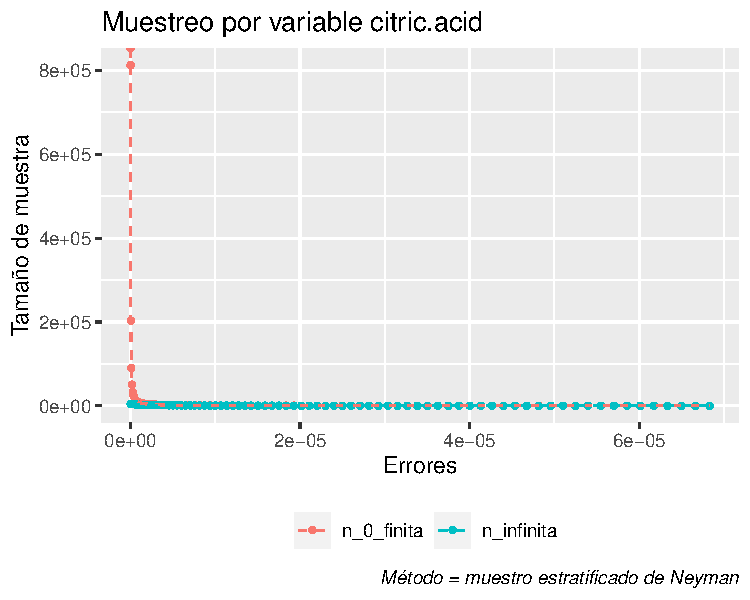
\includegraphics{muestreo_estratificado_final_files/figure-latex/grap uno de errores-1.pdf}
\caption{Gráfica de errores vs tamaños de población finita (azul) e
infinita (rosado)}
\end{figure}

De lo anterior es posible afirmar, sin tener encuenta otras variables
que van más allá de este análisis (recursos, economicas, logisticas,
entre otros), lo ideal es tomar el tamaño dónde se porduce la flexión de
la muestra para población finita y se aleja de la infinita para este
caso. Esto se puede afirmar porque el aplanamiento de la curva es
sostenido lo que quiere decir que independiente que se incremente el
tamaño de muestra en este punto el error seguirá siendo bajo, por lo
tanto considero que el tamaño de muestra adecuado para este caso sería
\(n=1024\).

\begin{figure}
\centering
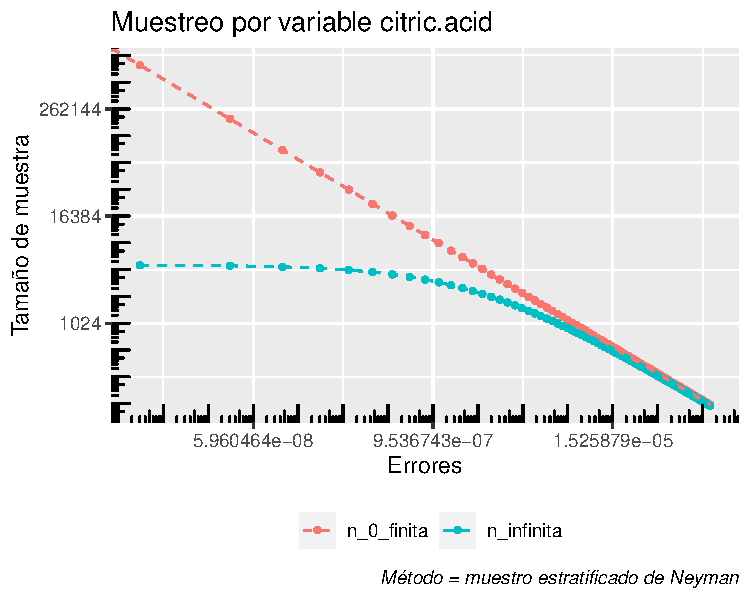
\includegraphics{muestreo_estratificado_final_files/figure-latex/grap uno de errores log2-1.pdf}
\caption{Gráfica de errores vs tamaños de población finita (azul) e
infinita (rosado) con transformación logaritmica (log2)}
\end{figure}

\hypertarget{estimadores-para-finales-para-variable-citric.acidy-totales}{%
\subsection{\texorpdfstring{Estimadores para finales para variable
\texttt{citric.acid}y
totales}{Estimadores para finales para variable citric.acidy totales}}\label{estimadores-para-finales-para-variable-citric.acidy-totales}}

\begin{table}[!h]

\caption{\label{tab:estimadores varianza estimada}Margenes de error y tamaños de población infinita y finita}
\centering
\fontsize{8}{10}\selectfont
\begin{tabular}[t]{c|c|c|c|c}
\hline
Estimadore & Media & Varianza & n & Varianza\_est\\
\hline
\rowcolor{gray!6}  dry & 0.3265714 & 0.008227009 & 140 & 472.69498\\
\hline
medium\_dry & 0.3219231 & 0.008961189 & 78 & 235.05416\\
\hline
\rowcolor{gray!6}  medium\_sweet & 0.3263636 & 0.008165455 & 11 & 37.45408\\
\hline
\multicolumn{5}{l}{\textit{Note: }}\\
\multicolumn{5}{l}{Se obtiene la varianza estimada para cada uno de los estratos}\\
\end{tabular}
\end{table}

\begin{table}[!h]

\caption{\label{tab:estimadores finales para la variable}Estimadores finales para la variable [citric.acid]}
\centering
\fontsize{8}{10}\selectfont
\begin{tabular}[t]{c|c|c|c|c}
\hline
Varianza\_est & ds\_estimada & Intervalo\_inf & Media\_est & Intervalo\_sup\\
\hline
\rowcolor{gray!6}  0.1610206 & 0.4012737 & -0.4774662 & 0.3250812 & 1.127629\\
\hline
\multicolumn{5}{l}{\textit{Note: }}\\
\multicolumn{5}{l}{sd = desviación estandar.}\\
\end{tabular}
\end{table}

Finalmente se decide realizar los estimadores finales para los estratos,
estos datos pueden ser observados en la tabla 10 y 11. En la primera se
puede observar la varianza estimada para cada uno de los estratos
respecto a la variable \texttt{citric.acid}. En el segundo se puede
observar los estimadores finales para la variable estudiada respecto a
la muestra final. Estos valores de muestra final son obtenidos a través
del remuestreo realizado por la función \texttt{strata}.

\begin{table}[!h]

\caption{\label{tab:estimadores finales totales}Estimadores totales para la variable [citric.acid]}
\centering
\fontsize{8}{10}\selectfont
\begin{tabular}[t]{c|c|c|c}
\hline
Varianza\_total & Intervalo\_inf & Media\_total & Intervalo\_sup\\
\hline
\rowcolor{gray!6}  745.2032 & 1449.879 & 1504.476 & 1582.051\\
\hline
\multicolumn{4}{l}{\textit{Note: }}\\
\multicolumn{4}{l}{Valores totales obtenidos a través de los estimadores}\\
\end{tabular}
\end{table}

\begin{table}[!h]

\caption{\label{tab:errores y tamaños de poblacion}Margenes de error y tamaños de población infinita y finita}
\centering
\fontsize{4}{6}\selectfont
\begin{tabular}[t]{c|c|c}
\hline
Margen de error & Muestra finita & muestra infinita\\
\hline
\rowcolor{gray!6}  0.00000e+00 & Inf & NaN\\
\hline
1.04000e-08 & 812228.9418 & 4601.7795\\
\hline
\rowcolor{gray!6}  4.17000e-08 & 203057.2354 & 4524.8709\\
\hline
9.37000e-08 & 90247.6602 & 4402.2479\\
\hline
\rowcolor{gray!6}  1.66600e-07 & 50764.3089 & 4241.3329\\
\hline
2.60300e-07 & 32489.1577 & 4050.9519\\
\hline
\rowcolor{gray!6}  3.74900e-07 & 22561.9150 & 3840.2673\\
\hline
5.10200e-07 & 16576.1009 & 3617.8943\\
\hline
\rowcolor{gray!6}  6.66400e-07 & 12691.0772 & 3391.3069\\
\hline
8.43400e-07 & 10027.5178 & 3166.5447\\
\hline
\rowcolor{gray!6}  1.04130e-06 & 8122.2894 & 2948.1649\\
\hline
1.25990e-06 & 6712.6359 & 2739.3595\\
\hline
\rowcolor{gray!6}  1.49940e-06 & 5640.4788 & 2542.1619\\
\hline
1.75970e-06 & 4806.0884 & 2357.6817\\
\hline
\rowcolor{gray!6}  2.04090e-06 & 4144.0252 & 2186.3308\\
\hline
2.34290e-06 & 3609.9064 & 2028.0210\\
\hline
\rowcolor{gray!6}  2.66570e-06 & 3172.7693 & 1882.3241\\
\hline
3.00930e-06 & 2810.4808 & 1748.5970\\
\hline
\rowcolor{gray!6}  3.37370e-06 & 2506.8794 & 1626.0735\\
\hline
3.75900e-06 & 2249.9417 & 1513.9311\\
\hline
\rowcolor{gray!6}  4.16510e-06 & 2030.5724 & 1411.3369\\
\hline
4.59200e-06 & 1841.7890 & 1317.4772\\
\hline
\rowcolor{gray!6}  5.03980e-06 & 1678.1590 & 1231.5769\\
\hline
5.50830e-06 & 1535.4044 & 1152.9102\\
\hline
\rowcolor{gray!6}  5.99770e-06 & 1410.1197 & 1080.8057\\
\hline
6.50790e-06 & 1299.5663 & 1014.6479\\
\hline
\rowcolor{gray!6}  7.03900e-06 & 1201.5221 & 953.8765\\
\hline
7.59090e-06 & 1114.1686 & 897.9835\\
\hline
\rowcolor{gray!6}  8.16360e-06 & 1036.0063 & 846.5099\\
\hline
8.75710e-06 & 965.7895 & 799.0422\\
\hline
\rowcolor{gray!6}  9.37140e-06 & 902.4766 & 755.2083\\
\hline
1.00066e-05 & 845.1914 & 714.6737\\
\hline
\rowcolor{gray!6}  1.06626e-05 & 793.1923 & 677.1378\\
\hline
1.13394e-05 & 745.8484 & 642.3305\\
\hline
\rowcolor{gray!6}  1.20371e-05 & 702.6202 & 610.0090\\
\hline
1.27556e-05 & 663.0440 & 579.9551\\
\hline
\rowcolor{gray!6}  1.34949e-05 & 626.7199 & 551.9722\\
\hline
1.42550e-05 & 593.3009 & 525.8836\\
\hline
\rowcolor{gray!6}  1.50360e-05 & 562.4854 & 501.5297\\
\hline
1.58377e-05 & 534.0098 & 478.7665\\
\hline
\rowcolor{gray!6}  1.66603e-05 & 507.6431 & 457.4641\\
\hline
1.75038e-05 & 483.1820 & 437.5047\\
\hline
\rowcolor{gray!6}  1.83680e-05 & 460.4472 & 418.7819\\
\hline
1.92531e-05 & 439.2801 & 401.1991\\
\hline
\rowcolor{gray!6}  2.01590e-05 & 419.5397 & 384.6686\\
\hline
2.10857e-05 & 401.1007 & 369.1105\\
\hline
\rowcolor{gray!6}  2.20333e-05 & 383.8511 & 354.4525\\
\hline
2.30017e-05 & 367.6908 & 340.6282\\
\hline
\rowcolor{gray!6}  2.39909e-05 & 352.5299 & 327.5773\\
\hline
2.50009e-05 & 338.2878 & 315.2447\\
\hline
\rowcolor{gray!6}  2.60318e-05 & 324.8916 & 303.5799\\
\hline
2.70835e-05 & 312.2756 & 292.5366\\
\hline
\rowcolor{gray!6}  2.81560e-05 & 300.3805 & 282.0726\\
\hline
2.92493e-05 & 289.1523 & 272.1488\\
\hline
\rowcolor{gray!6}  3.03635e-05 & 278.5422 & 262.7294\\
\hline
3.14985e-05 & 268.5054 & 253.7816\\
\hline
\rowcolor{gray!6}  3.26543e-05 & 259.0016 & 245.2750\\
\hline
3.38309e-05 & 249.9935 & 237.1815\\
\hline
\rowcolor{gray!6}  3.50284e-05 & 241.4474 & 229.4754\\
\hline
3.62466e-05 & 233.3321 & 222.1327\\
\hline
\rowcolor{gray!6}  3.74858e-05 & 225.6192 & 215.1313\\
\hline
3.87457e-05 & 218.2824 & 208.4507\\
\hline
\rowcolor{gray!6}  4.00265e-05 & 211.2979 & 202.0720\\
\hline
4.13280e-05 & 204.6432 & 195.9774\\
\hline
\rowcolor{gray!6}  4.26505e-05 & 198.2981 & 190.1506\\
\hline
4.39937e-05 & 192.2435 & 184.5764\\
\hline
\rowcolor{gray!6}  4.53578e-05 & 186.4621 & 179.2405\\
\hline
4.67427e-05 & 180.9376 & 174.1298\\
\hline
\rowcolor{gray!6}  4.81484e-05 & 175.6550 & 169.2319\\
\hline
4.95749e-05 & 170.6005 & 164.5353\\
\hline
\rowcolor{gray!6}  5.10223e-05 & 165.7610 & 160.0292\\
\hline
5.24905e-05 & 161.1246 & 155.7037\\
\hline
\rowcolor{gray!6}  5.39795e-05 & 156.6800 & 151.5493\\
\hline
5.54893e-05 & 152.4168 & 147.5572\\
\hline
\rowcolor{gray!6}  5.70200e-05 & 148.3252 & 143.7191\\
\hline
5.85715e-05 & 144.3963 & 140.0273\\
\hline
\rowcolor{gray!6}  6.01438e-05 & 140.6214 & 136.4746\\
\hline
6.17370e-05 & 136.9926 & 133.0541\\
\hline
\rowcolor{gray!6}  6.33509e-05 & 133.5025 & 129.7593\\
\hline
6.49857e-05 & 130.1440 & 126.5844\\
\hline
\rowcolor{gray!6}  6.66413e-05 & 126.9108 & 123.5235\\
\hline
6.83178e-05 & 123.7965 & 120.5713\\
\hline
\multicolumn{3}{l}{\textit{Note: }}\\
\multicolumn{3}{l}{El marge de error se obtuvo por la siquiente secuencia}\\
\multicolumn{3}{l}{seq(0,Error est, by=0.0002)}\\
\end{tabular}
\end{table}

\end{document}
